\section{System\-Data Class Reference}
\label{classSystemData}\index{SystemData@{SystemData}}
{\tt \#include $<$system.hpp$>$}

Collaboration diagram for System\-Data:\begin{figure}[H]
\begin{center}
\leavevmode
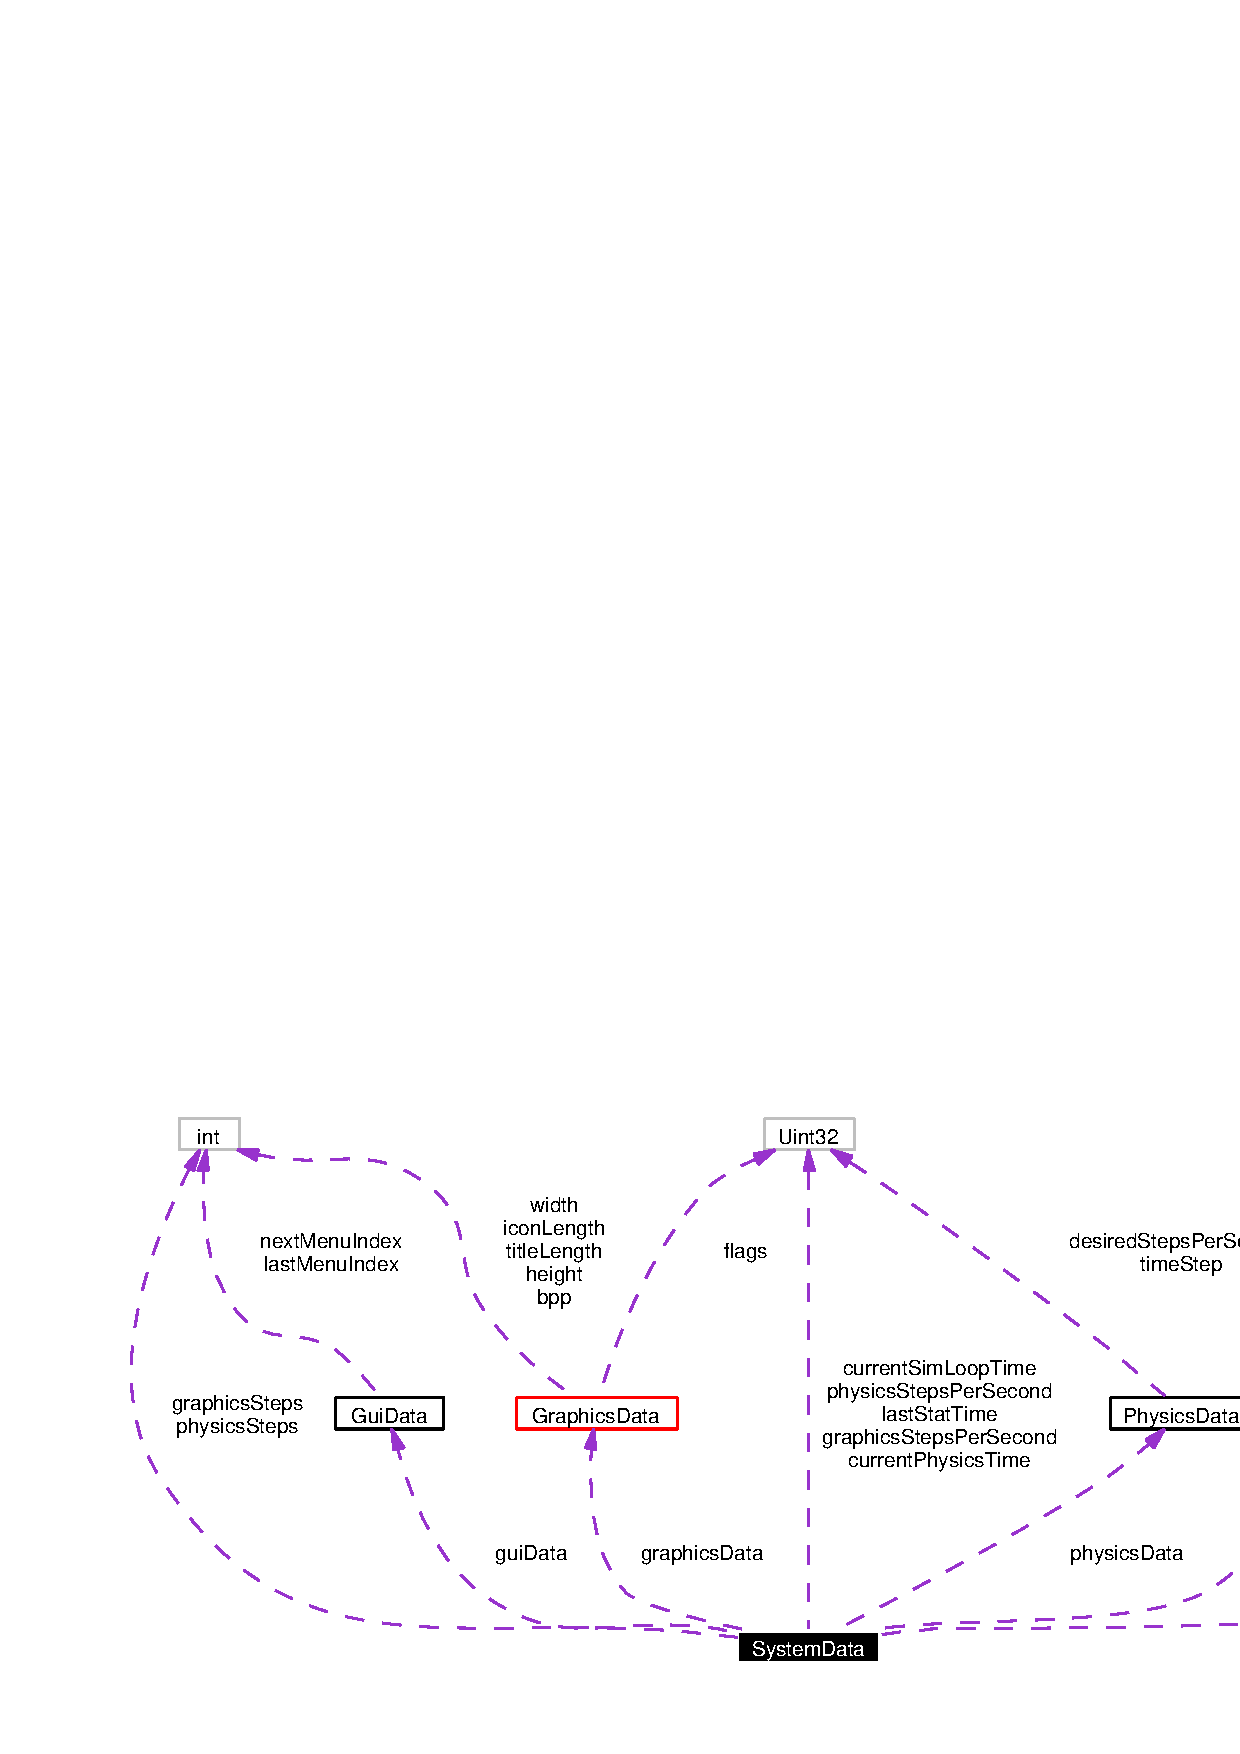
\includegraphics[width=397pt]{classSystemData__coll__graph}
\end{center}
\end{figure}
\subsection*{Public Member Functions}
\begin{CompactItemize}
\item 
bool {\bf can\-Main\-Loop\-Run} (void)
\item 
bool {\bf can\-Sim\-Loop\-Run} (void)
\item 
bool {\bf can\-Gui\-Loop\-Run} (void)
\item 
void {\bf enable\-Main\-Loop} (void)
\item 
void {\bf enable\-Sim\-Loop} (void)
\item 
void {\bf enable\-Gui\-Loop} (void)
\item 
void {\bf disable\-Main\-Loop} (void)
\item 
void {\bf disable\-Sim\-Loop} (void)
\item 
void {\bf disable\-Gui\-Loop} (void)
\end{CompactItemize}
\subsection*{Public Attributes}
\begin{CompactItemize}
\item 
{\bf Graphics\-Data} {\bf graphics\-Data}
\item 
{\bf Input\-Data} {\bf input\-Data}
\item 
{\bf Physics\-Data} {\bf physics\-Data}
\item 
{\bf Gui\-Data} {\bf gui\-Data}
\item 
Uint32 {\bf current\-Sim\-Loop\-Time}
\item 
Uint32 {\bf current\-Physics\-Time}
\item 
Uint32 {\bf last\-Stat\-Time}
\item 
int {\bf physics\-Steps}
\item 
Uint32 {\bf physics\-Steps\-Per\-Second}
\item 
int {\bf graphics\-Steps}
\item 
Uint32 {\bf graphics\-Steps\-Per\-Second}
\end{CompactItemize}
\subsection*{Private Attributes}
\begin{CompactItemize}
\item 
bool {\bf main\-Loop\-Enabled}
\item 
bool {\bf sim\-Loop\-Enabled}
\item 
bool {\bf gui\-Loop\-Enabled}
\end{CompactItemize}


\subsection{Member Function Documentation}
\index{SystemData@{System\-Data}!canGuiLoopRun@{canGuiLoopRun}}
\index{canGuiLoopRun@{canGuiLoopRun}!SystemData@{System\-Data}}
\subsubsection{\setlength{\rightskip}{0pt plus 5cm}bool System\-Data::can\-Gui\-Loop\-Run (void)}\label{classSystemData_a2}


\index{SystemData@{System\-Data}!canMainLoopRun@{canMainLoopRun}}
\index{canMainLoopRun@{canMainLoopRun}!SystemData@{System\-Data}}
\subsubsection{\setlength{\rightskip}{0pt plus 5cm}bool System\-Data::can\-Main\-Loop\-Run (void)}\label{classSystemData_a0}


\index{SystemData@{System\-Data}!canSimLoopRun@{canSimLoopRun}}
\index{canSimLoopRun@{canSimLoopRun}!SystemData@{System\-Data}}
\subsubsection{\setlength{\rightskip}{0pt plus 5cm}bool System\-Data::can\-Sim\-Loop\-Run (void)}\label{classSystemData_a1}


\index{SystemData@{System\-Data}!disableGuiLoop@{disableGuiLoop}}
\index{disableGuiLoop@{disableGuiLoop}!SystemData@{System\-Data}}
\subsubsection{\setlength{\rightskip}{0pt plus 5cm}void System\-Data::disable\-Gui\-Loop (void)}\label{classSystemData_a8}


\index{SystemData@{System\-Data}!disableMainLoop@{disableMainLoop}}
\index{disableMainLoop@{disableMainLoop}!SystemData@{System\-Data}}
\subsubsection{\setlength{\rightskip}{0pt plus 5cm}void System\-Data::disable\-Main\-Loop (void)}\label{classSystemData_a6}


\index{SystemData@{System\-Data}!disableSimLoop@{disableSimLoop}}
\index{disableSimLoop@{disableSimLoop}!SystemData@{System\-Data}}
\subsubsection{\setlength{\rightskip}{0pt plus 5cm}void System\-Data::disable\-Sim\-Loop (void)}\label{classSystemData_a7}


\index{SystemData@{System\-Data}!enableGuiLoop@{enableGuiLoop}}
\index{enableGuiLoop@{enableGuiLoop}!SystemData@{System\-Data}}
\subsubsection{\setlength{\rightskip}{0pt plus 5cm}void System\-Data::enable\-Gui\-Loop (void)}\label{classSystemData_a5}


\index{SystemData@{System\-Data}!enableMainLoop@{enableMainLoop}}
\index{enableMainLoop@{enableMainLoop}!SystemData@{System\-Data}}
\subsubsection{\setlength{\rightskip}{0pt plus 5cm}void System\-Data::enable\-Main\-Loop (void)}\label{classSystemData_a3}


\index{SystemData@{System\-Data}!enableSimLoop@{enableSimLoop}}
\index{enableSimLoop@{enableSimLoop}!SystemData@{System\-Data}}
\subsubsection{\setlength{\rightskip}{0pt plus 5cm}void System\-Data::enable\-Sim\-Loop (void)}\label{classSystemData_a4}




\subsection{Member Data Documentation}
\index{SystemData@{System\-Data}!currentPhysicsTime@{currentPhysicsTime}}
\index{currentPhysicsTime@{currentPhysicsTime}!SystemData@{System\-Data}}
\subsubsection{\setlength{\rightskip}{0pt plus 5cm}Uint32 {\bf System\-Data::current\-Physics\-Time}}\label{classSystemData_o5}


\index{SystemData@{System\-Data}!currentSimLoopTime@{currentSimLoopTime}}
\index{currentSimLoopTime@{currentSimLoopTime}!SystemData@{System\-Data}}
\subsubsection{\setlength{\rightskip}{0pt plus 5cm}Uint32 {\bf System\-Data::current\-Sim\-Loop\-Time}}\label{classSystemData_o4}


\index{SystemData@{System\-Data}!graphicsData@{graphicsData}}
\index{graphicsData@{graphicsData}!SystemData@{System\-Data}}
\subsubsection{\setlength{\rightskip}{0pt plus 5cm}struct {\bf Graphics\-Data} {\bf System\-Data::graphics\-Data}}\label{classSystemData_o0}


\index{SystemData@{System\-Data}!graphicsSteps@{graphicsSteps}}
\index{graphicsSteps@{graphicsSteps}!SystemData@{System\-Data}}
\subsubsection{\setlength{\rightskip}{0pt plus 5cm}int {\bf System\-Data::graphics\-Steps}}\label{classSystemData_o9}


\index{SystemData@{System\-Data}!graphicsStepsPerSecond@{graphicsStepsPerSecond}}
\index{graphicsStepsPerSecond@{graphicsStepsPerSecond}!SystemData@{System\-Data}}
\subsubsection{\setlength{\rightskip}{0pt plus 5cm}Uint32 {\bf System\-Data::graphics\-Steps\-Per\-Second}}\label{classSystemData_o10}


\index{SystemData@{System\-Data}!guiData@{guiData}}
\index{guiData@{guiData}!SystemData@{System\-Data}}
\subsubsection{\setlength{\rightskip}{0pt plus 5cm}struct {\bf Gui\-Data} {\bf System\-Data::gui\-Data}}\label{classSystemData_o3}


\index{SystemData@{System\-Data}!guiLoopEnabled@{guiLoopEnabled}}
\index{guiLoopEnabled@{guiLoopEnabled}!SystemData@{System\-Data}}
\subsubsection{\setlength{\rightskip}{0pt plus 5cm}bool {\bf System\-Data::gui\-Loop\-Enabled}\hspace{0.3cm}{\tt  [private]}}\label{classSystemData_r2}


\index{SystemData@{System\-Data}!inputData@{inputData}}
\index{inputData@{inputData}!SystemData@{System\-Data}}
\subsubsection{\setlength{\rightskip}{0pt plus 5cm}struct {\bf Input\-Data} {\bf System\-Data::input\-Data}}\label{classSystemData_o1}


\index{SystemData@{System\-Data}!lastStatTime@{lastStatTime}}
\index{lastStatTime@{lastStatTime}!SystemData@{System\-Data}}
\subsubsection{\setlength{\rightskip}{0pt plus 5cm}Uint32 {\bf System\-Data::last\-Stat\-Time}}\label{classSystemData_o6}


\index{SystemData@{System\-Data}!mainLoopEnabled@{mainLoopEnabled}}
\index{mainLoopEnabled@{mainLoopEnabled}!SystemData@{System\-Data}}
\subsubsection{\setlength{\rightskip}{0pt plus 5cm}bool {\bf System\-Data::main\-Loop\-Enabled}\hspace{0.3cm}{\tt  [private]}}\label{classSystemData_r0}


\index{SystemData@{System\-Data}!physicsData@{physicsData}}
\index{physicsData@{physicsData}!SystemData@{System\-Data}}
\subsubsection{\setlength{\rightskip}{0pt plus 5cm}struct {\bf Physics\-Data} {\bf System\-Data::physics\-Data}}\label{classSystemData_o2}


\index{SystemData@{System\-Data}!physicsSteps@{physicsSteps}}
\index{physicsSteps@{physicsSteps}!SystemData@{System\-Data}}
\subsubsection{\setlength{\rightskip}{0pt plus 5cm}int {\bf System\-Data::physics\-Steps}}\label{classSystemData_o7}


\index{SystemData@{System\-Data}!physicsStepsPerSecond@{physicsStepsPerSecond}}
\index{physicsStepsPerSecond@{physicsStepsPerSecond}!SystemData@{System\-Data}}
\subsubsection{\setlength{\rightskip}{0pt plus 5cm}Uint32 {\bf System\-Data::physics\-Steps\-Per\-Second}}\label{classSystemData_o8}


\index{SystemData@{System\-Data}!simLoopEnabled@{simLoopEnabled}}
\index{simLoopEnabled@{simLoopEnabled}!SystemData@{System\-Data}}
\subsubsection{\setlength{\rightskip}{0pt plus 5cm}bool {\bf System\-Data::sim\-Loop\-Enabled}\hspace{0.3cm}{\tt  [private]}}\label{classSystemData_r1}




The documentation for this class was generated from the following files:\begin{CompactItemize}
\item 
src/{\bf system.hpp}\item 
src/{\bf system.cpp}\end{CompactItemize}
